\documentclass[12pt,a4paper]{article}
\usepackage[utf8]{inputenc}
\usepackage[spanish]{babel}
\usepackage{graphicx}
\usepackage{kpfonts}
\usepackage[left=2cm,right=2cm,top=2cm,bottom=2cm]{geometry}
\author{Jorge Bueno}
\begin{document}
\title{\textbf{Universidad Politecnica \\ de la \\ Zona Metropolitana de Guadalajara}}
\author{\textbf{Practica 7} Construir un amplificacion con conexion Darlington\\Jorge Heriberto Bueno Gomez \\Amairani Ivette Marquez Marquez\\Ing. Mecatronica 4 B}
\maketitle
$$
\includegraphics[scale=.5]{UPCDLZMDG5783-logo.png} $$
\newpage
\section{Ojetivo} 
Controlar un Relay con un Ldr utilizando un darlington tip 112. 
Tambien controlar el circuito anterios del desarrollo del plc pero sustituyendo el 2N2222 por un TIP 112.

\section{Materiales}
\begin{tabular}{|c|}
\hline 
\textbf{Materiales }\\ 
\hline 
Ldr \\ 
\hline 
TIP112 \\ 
\hline 
Relay \\ 
\hline 
Resistencia 100K \\ 
\hline 
Diodo shottky \\ 
\hline 
\end{tabular} 
\section{Marco teorico}
\subsection{LDR}
El LDR por sus siglas en inglés (Light Dependent Resistor) o fotoresistor es una resistencia la cual varía su valor en función de la cantidad de luz que incide sobre su superficie. Cuanto mayor sea la intensidad de luz que incide en la superficie del LDR o fotoresistor menor será su resistencia y en cuanto menor sea la luz que incida sobre éste mayor será su resistencia.

\subsection{TIP 112}
Transistor TIP112 con Darlington de silicio epitexial de polaridad NPN que cuenta con una construcción monolítica con resistencias de derivación base-emisor incorporadas. Es complementario a los transistores TIP115 / TIP116 / TIP117. Cuenta con bajo voltaje de saturación de colector-emisor.


    • Alta ganancia de corriente continua\\
    • Con diodo Darlington\\
    • Aplicaciones: Industrial\\
\textbf{Información Básica}\\
    • Polaridad del transistor: NPN\\
    • Voltaje colector emisor V (br) ceo: 100 V\\
    • Caída de Voltaje: 100 V\\
    • Disipación de potencia Pd: 50 W\\
    • Corriente del colector DC: 2 A\\
    • Ganancia de corriente DC hFE: 1000 hFE\\
    • Temperatura de trabajo máxima: 150°C\\
    • Encapsulado: TO-220\\
    • 3 pines\\


\section{Procedimiento}
Primero analizamos el circuito a armar.\\
Despues seleccionamos los componentes a utilizar.\\
Por ultimo armamos el circuito y lo checamos.\\
\section{Resultados}
$$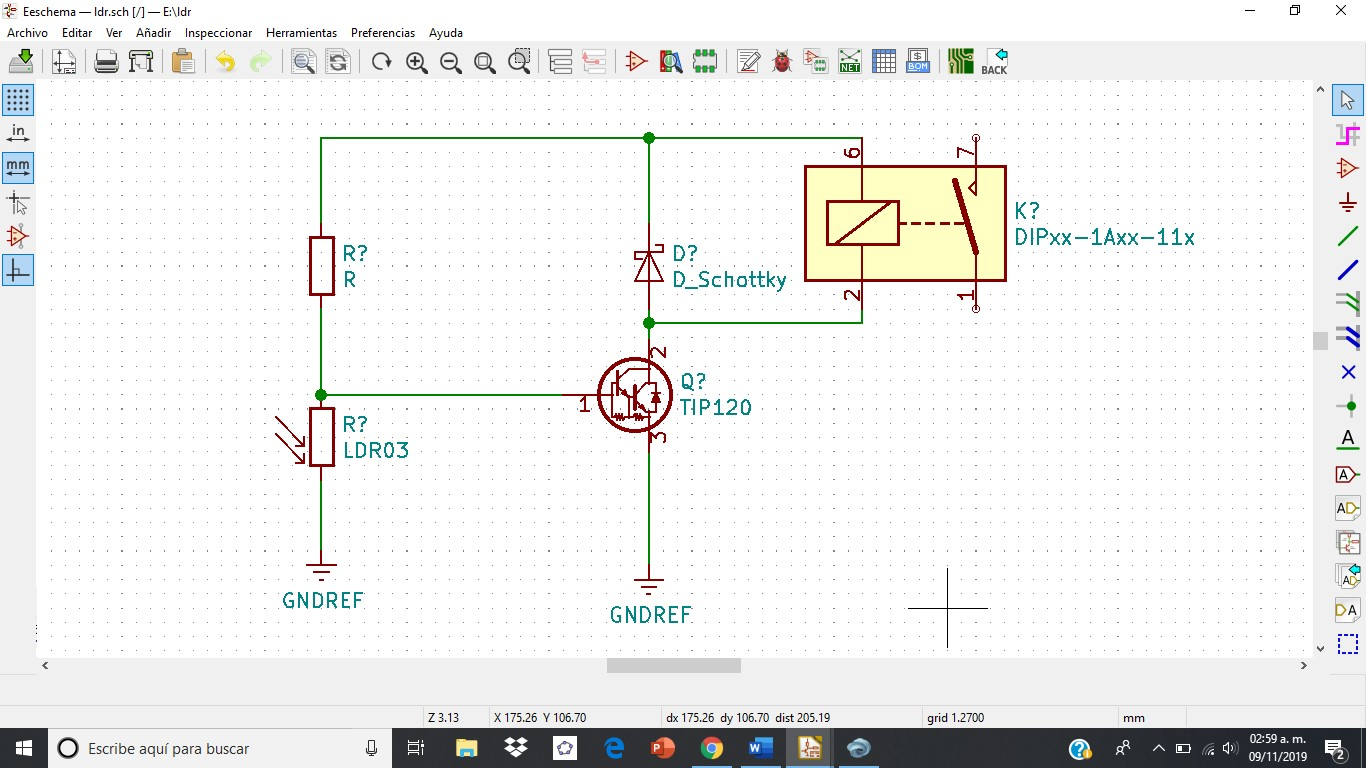
\includegraphics[scale=.5]{1.jpg}$$
$$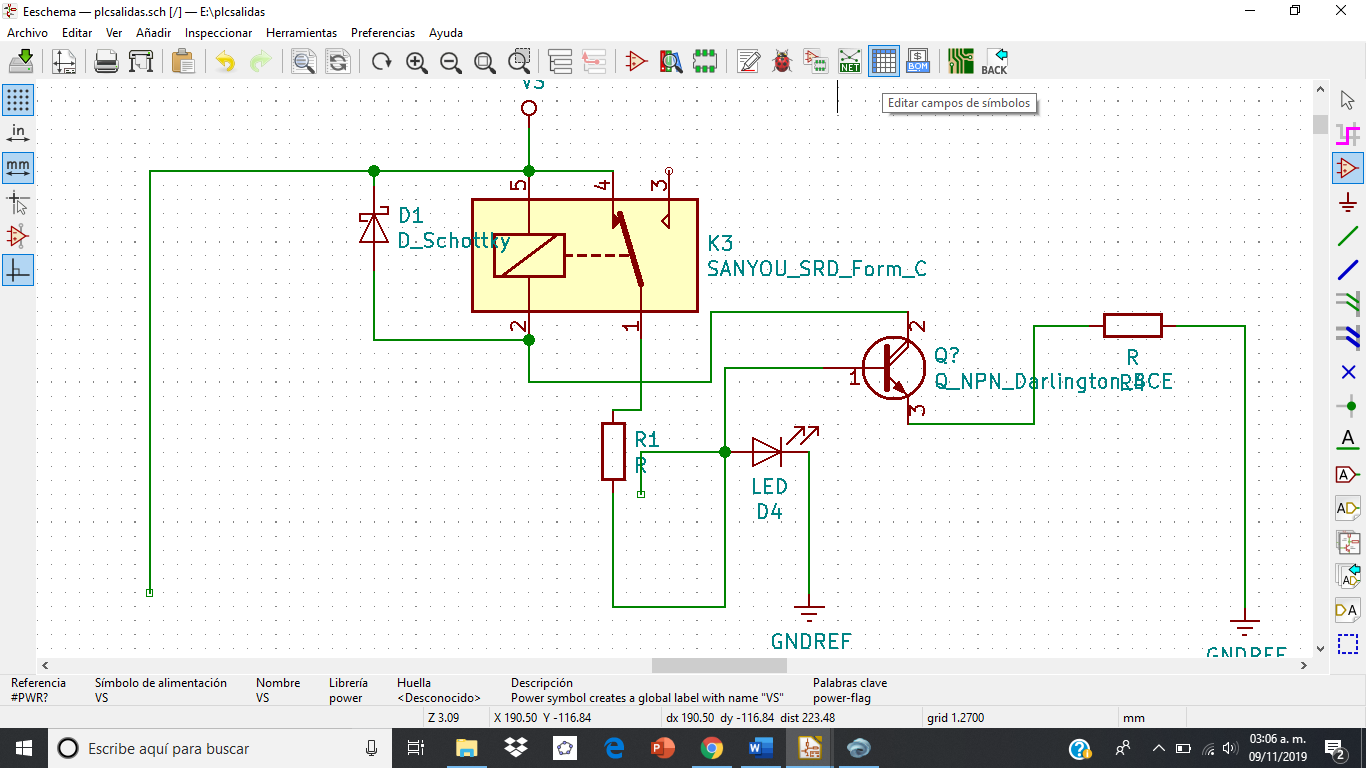
\includegraphics[scale=.5]{2.png} $$
$$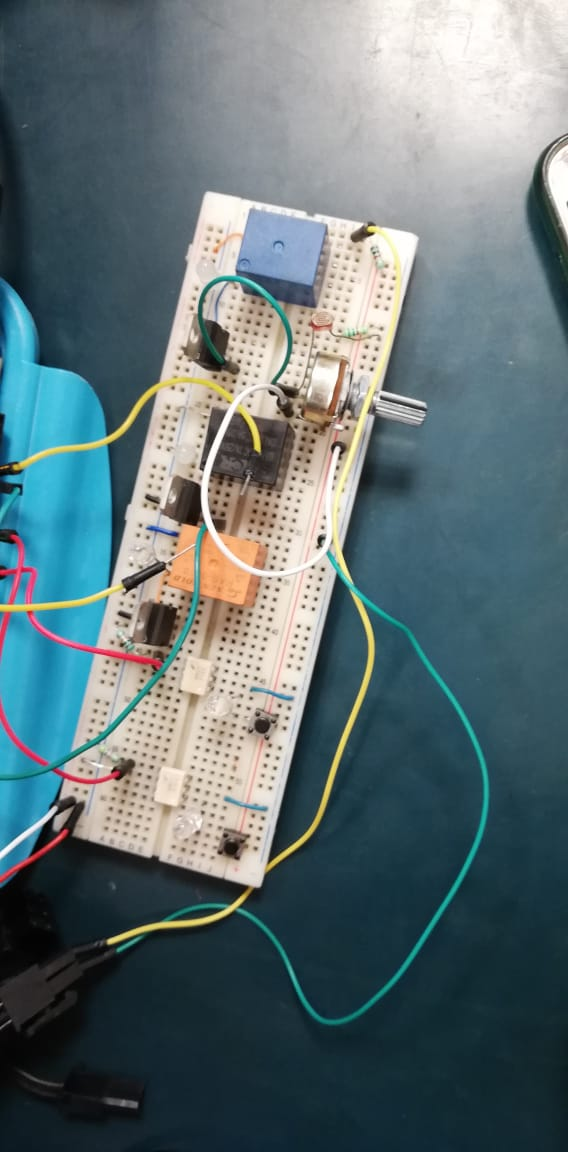
\includegraphics[scale=.2]{4.jpg} $$ 
\section{Conclusion}
En esta practica aprendimos el funcionamiento del LDR y mas que nada la practica se baso en el TIP 112 que es un transistor Darlington que se puede usar con altos voltajes como lo hicimos con un contactor de 24 voltion pero usando el arduino.
\end{document} 